\documentclass[11pt,a4paper]{article}

% ── Core packages ─────────────────────────────────────────────────────────────
\usepackage[utf8]{inputenc}
\usepackage[T1]{fontenc}
\usepackage{lmodern}
\usepackage[margin=2.2cm,top=2.8cm,bottom=2.5cm]{geometry}
\usepackage{xcolor}
\usepackage[most]{tcolorbox}
\usepackage{titlesec}
\usepackage{enumitem}
\usepackage{booktabs}
\usepackage{array}
\usepackage{tabularx}
\usepackage{fancyhdr}
\usepackage{listings}
\usepackage[hidelinks]{hyperref}
\usepackage{tikz}
\usetikzlibrary{arrows.meta,positioning,backgrounds,calc}
\usepackage{float}
\usepackage{caption}
\usepackage{amsmath}
\usepackage{amssymb}
\usepackage{microtype}

% ── Color palette ─────────────────────────────────────────────────────────────
\definecolor{spInk}{HTML}{1F2A44}
\definecolor{spPrimary}{HTML}{2A4D9B}
\definecolor{spAccent}{HTML}{0E7C7B}
\definecolor{spHow}{HTML}{1565C0}
\definecolor{spWhy}{HTML}{2E7D32}
\definecolor{spSec}{HTML}{B23A00}
\definecolor{spQA}{HTML}{5E35B1}
\definecolor{spGrayBg}{HTML}{F4F6FB}
\definecolor{spRule}{HTML}{C9D2E8}
\definecolor{spLightBlue}{HTML}{E3F2FD}
\definecolor{spLightGreen}{HTML}{E8F5E9}
\definecolor{spLightPurple}{HTML}{EDE7F6}
\definecolor{spLightOrange}{HTML}{FBE9E7}
\definecolor{spLightTeal}{HTML}{E0F2F1}
\definecolor{spLightYellow}{HTML}{FFF9C4}
\definecolor{spYellow}{HTML}{F9A825}
\definecolor{spOrange}{HTML}{E65100}

% ── Typography ────────────────────────────────────────────────────────────────
\hypersetup{colorlinks=true,linkcolor=spPrimary,urlcolor=spAccent,
  pdftitle={ScholarPath AI Architecture Deep Dive},
  pdfauthor={ScholarPath Graduation Project}}
\titleformat{\section}{\Large\bfseries\color{spPrimary}}{\thesection.}{0.5em}{}
\titleformat{\subsection}{\large\bfseries\color{spAccent}}{\thesubsection}{0.5em}{}
\titleformat{\subsubsection}{\normalsize\bfseries\color{spInk}}{\thesubsubsection}{0.5em}{}
\titlespacing*{\section}{0pt}{18pt}{6pt}
\titlespacing*{\subsection}{0pt}{12pt}{4pt}
\setlist{nosep,leftmargin=1.5em,topsep=2pt}

% ── Header / Footer ───────────────────────────────────────────────────────────
\pagestyle{fancy}\fancyhf{}
\renewcommand{\headrulewidth}{0.4pt}
\fancyhead[L]{\small\color{spPrimary}\textbf{ScholarPath}}
\fancyhead[R]{\small\color{spInk}AI Architecture Deep Dive}
\fancyfoot[C]{\small\thepage}

% ── tcolorbox environments ────────────────────────────────────────────────────
\newtcolorbox{conceptbox}[1]{breakable,
  colback=spLightBlue,colframe=spHow!75!black,boxrule=0.7pt,arc=2pt,
  left=6pt,right=6pt,top=4pt,bottom=4pt,
  fonttitle=\bfseries\color{white},colbacktitle=spHow,
  title=\textsc{Concept: #1}}

\newtcolorbox{whybox}{breakable,
  colback=spLightGreen,colframe=spWhy!70!black,boxrule=0.7pt,arc=2pt,
  left=6pt,right=6pt,top=4pt,bottom=4pt,
  fonttitle=\bfseries\color{white},colbacktitle=spWhy!80!black,
  title=Why this design?}

\newtcolorbox{keybox}[1]{breakable,
  colback=spLightPurple,colframe=spQA!70!black,boxrule=0.7pt,arc=2pt,
  left=6pt,right=6pt,top=4pt,bottom=4pt,
  fonttitle=\bfseries\color{white},colbacktitle=spQA!80!black,
  title=\textsc{Key Point: #1}}

\newtcolorbox{warningbox}{breakable,
  colback=spLightOrange,colframe=spSec!70!black,boxrule=0.7pt,arc=2pt,
  left=6pt,right=6pt,top=4pt,bottom=4pt,
  fonttitle=\bfseries\color{white},colbacktitle=spSec!80!black,
  title=Important Note}

\newtcolorbox{notebox}{breakable,
  colback=spLightTeal,colframe=spAccent!70!black,boxrule=0.7pt,arc=2pt,
  left=6pt,right=6pt,top=4pt,bottom=4pt,
  fonttitle=\bfseries\color{white},colbacktitle=spAccent!80!black,
  title=Note}

% ── Code listing ──────────────────────────────────────────────────────────────
\lstset{basicstyle=\ttfamily\footnotesize,
  backgroundcolor=\color{spGrayBg},frame=single,rulecolor=\color{spRule},
  breaklines=true,breakatwhitespace=true,tabsize=4,
  keywordstyle=\color{spPrimary}\bfseries,
  commentstyle=\color{spWhy}\itshape,
  stringstyle=\color{spSec},
  showstringspaces=false,
  xleftmargin=4pt,framexleftmargin=2pt}

% ── TikZ node styles (ALL use rectangle + text width for reliable \\) ─────────
\tikzset{
  % Blue process box
  pbox/.style={rectangle,rounded corners=4pt,
    text width=2.7cm,minimum height=0.78cm,
    align=center,draw=spPrimary!65,fill=spLightBlue,
    font=\small\bfseries,text=spPrimary!80},
  % Light step box
  sbox/.style={rectangle,rounded corners=3pt,
    text width=2.7cm,minimum height=0.72cm,
    align=center,draw=spPrimary!40,fill=spGrayBg,
    font=\small,text=spInk},
  % GPT / LLM box (purple)
  gbox/.style={rectangle,rounded corners=4pt,
    text width=2.7cm,minimum height=0.78cm,
    align=center,draw=spQA!70,fill=spLightPurple,
    font=\small\bfseries,text=spQA!80},
  % Fallback box (orange)
  fbox/.style={rectangle,rounded corners=3pt,
    text width=2.7cm,minimum height=0.72cm,
    align=center,draw=spSec!65,fill=spLightOrange,
    font=\small,text=spSec!80},
  % Source box (green)
  srcbox/.style={rectangle,rounded corners=4pt,
    text width=2.6cm,minimum height=0.65cm,
    align=center,draw=spWhy!60,fill=spLightGreen,
    font=\scriptsize,text=spWhy!80},
  % Database box (teal, double border)
  dbbox/.style={rectangle,rounded corners=3pt,
    text width=2.0cm,minimum height=0.78cm,
    align=center,draw=spAccent!70,fill=spLightTeal,
    font=\small\bfseries,text=spAccent!80,
    double,double distance=1.4pt},
  % Decision box (yellow)
  dbox/.style={rectangle,rounded corners=2pt,
    text width=2.6cm,minimum height=0.68cm,
    align=center,draw=spYellow!85!black,fill=spLightYellow,
    font=\scriptsize\itshape,text=spOrange!90},
  % Wide pipeline step (full width)
  wbox/.style={rectangle,rounded corners=3pt,
    text width=11.4cm,minimum height=0.68cm,
    align=center,draw=spPrimary!35,fill=spGrayBg,
    font=\small,text=spInk},
  % Arrows
  arr/.style={->,>=Stealth,semithick,color=spInk!55},
  arrd/.style={->,>=Stealth,semithick,dashed,color=spInk!35},
  lbl/.style={font=\scriptsize,text=spInk!55},
}

\captionsetup{font=small,labelfont=bf,labelsep=period}

% ═════════════════════════════════════════════════════════════════════════════
\begin{document}
% ═════════════════════════════════════════════════════════════════════════════

% ── Cover ─────────────────────────────────────────────────────────────────────
\begin{tcolorbox}[colback=spPrimary,colframe=spPrimary,arc=4pt,boxrule=0pt]
  \color{white}
  {\Huge\bfseries ScholarPath}\\[3pt]
  {\LARGE AI Architecture Deep Dive}\\[8pt]
  {\normalsize Retrieval-Augmented Generation, Rule-Based Scoring \& Eligibility
  Checking --- a comprehensive technical reference for the academic defence.
  Every diagram and code snippet reflects the live production codebase.}
\end{tcolorbox}

\vspace{4pt}
{\small\color{spInk}
\textbf{Stack:} .NET 10 \textperiodcentered{} React 19 \textperiodcentered{}
Azure OpenAI (gpt-4o-mini + text-embedding-3-small) \textperiodcentered{}
SQL Server \textperiodcentered{} 692 KB documents \textperiodcentered{}
Standard RAG (not Agentic).}

\vspace{2pt}\hrule height 0.4pt\vspace{6pt}
{\small\tableofcontents}
\vspace{4pt}\hrule height 0.4pt

\newpage

% ═════════════════════════════════════════════════════════════════════════════
\section{Core Concepts}
% ═════════════════════════════════════════════════════════════════════════════

\subsection{Embeddings --- Turning Text into Numbers}

\begin{conceptbox}{Embedding}
An \textbf{embedding} converts any text --- a word, sentence, or paragraph ---
into a fixed-length array of floating-point numbers called a \emph{vector}.
The fundamental property: \textbf{semantically similar texts produce numerically
close vectors}, regardless of exact wording or even language.
A question in English and the same question in Arabic yield vectors that point
in nearly the same direction in a 1,536-dimensional space.
\end{conceptbox}

\begin{figure}[H]
\centering
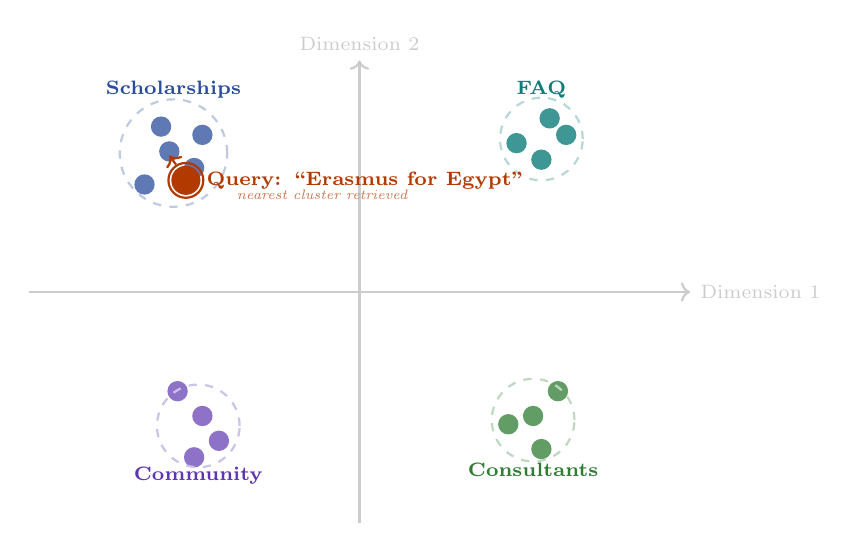
\begin{tikzpicture}[scale=1.05]
  % Axes
  \draw[->,gray!40,thick] (-4,0) -- (4,0)
    node[right,font=\scriptsize,gray!40] {Dimension 1};
  \draw[->,gray!40,thick] (0,-2.8) -- (0,2.8)
    node[above,font=\scriptsize,gray!40] {Dimension 2};

  % Cluster: Scholarships (blue)
  \foreach \x/\y in {-2.3/1.7,-2.6/1.3,-2.0/1.5,-2.4/2.0,-1.9/1.9}
    \fill[spPrimary!75] (\x,\y) circle(3.5pt);
  \draw[spPrimary!30,dashed,thick] (-2.25,1.68) circle(0.65cm);
  \node[font=\scriptsize\bfseries,color=spPrimary] at (-2.25,2.45) {Scholarships};

  % Cluster: FAQ (teal)
  \foreach \x/\y in {2.2/1.6,2.5/1.9,1.9/1.8,2.3/2.1}
    \fill[spAccent!80] (\x,\y) circle(3.5pt);
  \draw[spAccent!30,dashed,thick] (2.2,1.85) circle(0.5cm);
  \node[font=\scriptsize\bfseries,color=spAccent] at (2.2,2.45) {FAQ};

  % Cluster: Consultants (green)
  \foreach \x/\y in {2.1/-1.5,2.4/-1.2,1.8/-1.6,2.2/-1.9}
    \fill[spWhy!75] (\x,\y) circle(3.5pt);
  \draw[spWhy!30,dashed,thick] (2.1,-1.55) circle(0.5cm);
  \node[font=\scriptsize\bfseries,color=spWhy] at (2.1,-2.15) {Consultants};

  % Cluster: Community (purple)
  \foreach \x/\y in {-1.9/-1.5,-2.2/-1.2,-1.7/-1.8,-2.0/-2.0}
    \fill[spQA!70] (\x,\y) circle(3.5pt);
  \draw[spQA!30,dashed,thick] (-1.95,-1.62) circle(0.5cm);
  \node[font=\scriptsize\bfseries,color=spQA] at (-1.95,-2.22) {Community};

  % Query star (red dot)
  \fill[spSec] (-2.1,1.35) circle(5pt);
  \draw[spSec,thick] (-2.1,1.35) circle(6pt);
  \node[font=\scriptsize\bfseries,color=spSec,right=4pt] at (-2.1,1.35)
    {Query: ``Erasmus for Egypt''};

  % Nearest-neighbor arrow
  \draw[->,spSec,thick,dashed] (-2.1,1.38) -- (-2.3,1.65);
  \node[font=\tiny,color=spSec!70,above right] at (-1.6,1.0)
    {\textit{nearest cluster retrieved}};
\end{tikzpicture}
\caption{Conceptual 2-D embedding space (real vectors have 1,536 dimensions). The query
  vector (red circle) lands near the Scholarship cluster. The retriever returns those docs
  as context for the LLM.}
\end{figure}

In ScholarPath the embedding model is \textbf{Azure OpenAI \texttt{text-embedding-3-small}}
producing \textbf{1,536-dimensional} vectors. A \texttt{sp:} prefix namespaces the model
name in the database so vectors from different models are never mixed in search:

\begin{lstlisting}[language={[Sharp]C},caption={AzureOpenAiEmbeddingService.cs --- ModelName}]
public string ModelName =>
    IsAzureEmbeddingConfigured()
        ? $"sp:{opts.Value.AzureOpenAi.EmbeddingDeploymentName}"
        // ^ "sp:text-embedding-3-small" -- sp: is a namespace prefix only
        : local.ModelName;   // fallback when Azure is not configured
\end{lstlisting}

% ─────────────────────────────────────────────────────────────────────────────
\subsection{Cosine Similarity --- Measuring Semantic Closeness}

Given two embedding vectors $\mathbf{a}$ and $\mathbf{b}$, cosine similarity
measures the \emph{angle} between them (not their lengths):

\[
\cos(\theta)
= \frac{\mathbf{a}\cdot\mathbf{b}}{\|\mathbf{a}\|\;\|\mathbf{b}\|}
= \frac{\displaystyle\sum_{i=1}^{n}a_i b_i}
       {\displaystyle\sqrt{\sum_{i=1}^{n}a_i^2}\;\sqrt{\sum_{i=1}^{n}b_i^2}}
\quad\in[0,\,1]
\]

\begin{figure}[H]
\centering
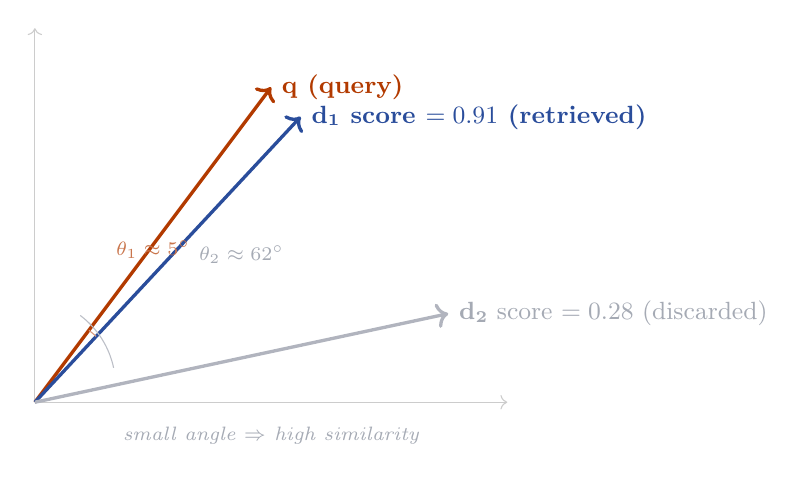
\begin{tikzpicture}[scale=1.25]
  \draw[->,gray!40] (0,0) -- (4.8,0);
  \draw[->,gray!40] (0,0) -- (0,3.8);

  % Query
  \draw[->,spSec,very thick] (0,0) -- (2.4,3.2)
    node[right,font=\small\bfseries,color=spSec] {$\mathbf{q}$ (query)};

  % Similar doc (small angle)
  \draw[->,spPrimary,very thick] (0,0) -- (2.7,2.9)
    node[right,font=\small\bfseries,color=spPrimary]
    {$\mathbf{d_1}$ score $= 0.91$ (retrieved)};

  % Dissimilar doc (large angle)
  \draw[->,spInk!35,very thick] (0,0) -- (4.2,0.9)
    node[right,font=\small,color=spInk!40]
    {$\mathbf{d_2}$ score $= 0.28$ (discarded)};

  % Angle arcs
  \draw[spSec!50,thin]
    (0.55,0.73) arc[start angle=53,end angle=47,radius=0.9cm];
  \node[font=\scriptsize,color=spSec!70] at (1.2,1.55)
    {$\theta_1 \approx 5{}^{\circ}$};

  \draw[spInk!30,thin]
    (0.8,0.35) arc[start angle=12,end angle=53,radius=0.9cm];
  \node[font=\scriptsize,color=spInk!40] at (2.1,1.5)
    {$\theta_2 \approx 62{}^{\circ}$};

  \node[font=\scriptsize\itshape,color=spInk!40,below] at (2.4,-0.15)
    {small angle $\Rightarrow$ high similarity};
\end{tikzpicture}
\caption{Two documents against a query. $\mathbf{d_1}$ (small angle, score 0.91) lies above
  the \texttt{RagMinScore = 0.6} threshold and is included in the LLM context block.
  $\mathbf{d_2}$ is discarded.}
\end{figure}

\begin{center}
\begin{tabular}{clp{7cm}}
\toprule
\textbf{Score} & \textbf{Interpretation} & \textbf{Action in ScholarPath}\\
\midrule
$\geq 0.85$ & Near-identical meaning & Retrieved \& cited in response\\
$0.70$--$0.84$ & Very similar & Retrieved \& cited\\
$0.60$--$0.69$ & Clearly related & Retrieved (at \texttt{RagMinScore} threshold)\\
$<0.60$ & Weakly related & Discarded before LLM prompt\\
\bottomrule
\end{tabular}
\end{center}

% ─────────────────────────────────────────────────────────────────────────────
\subsection{What is RAG?}

\begin{conceptbox}{Retrieval-Augmented Generation (RAG)}
RAG solves the \emph{knowledge gap} of LLMs. Instead of answering purely from
training memory (which may be stale or hallucinated), the LLM receives
\textbf{retrieved, grounded context} from a live knowledge base alongside the
user's question. The context anchors the answer to real, up-to-date data.
\end{conceptbox}

\begin{figure}[H]
\centering
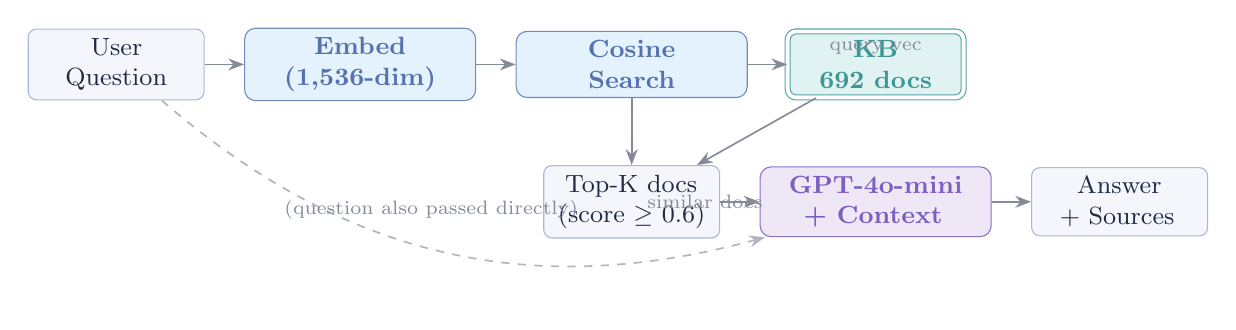
\begin{tikzpicture}[node distance=0.3cm and 0.5cm]
  \node[sbox,text width=2.0cm] (q) {User\\Question};
  \node[pbox,right=0.5cm of q] (emb) {Embed\\(1,536-dim)};
  \node[pbox,right=0.5cm of emb] (srch) {Cosine\\Search};
  \node[dbbox,right=0.5cm of srch] (kb) {KB\\692 docs};
  \node[sbox,text width=2.0cm,below=0.85cm of srch] (topk)
    {Top-K docs\\(score $\geq$ 0.6)};
  \node[gbox,right=0.5cm of topk] (llm) {GPT-4o-mini\\+ Context};
  \node[sbox,text width=2.0cm,right=0.5cm of llm] (ans)
    {Answer\\+ Sources};

  \draw[arr] (q) -- (emb);
  \draw[arr] (emb) -- (srch);
  \draw[arr] (srch) -- (kb) node[lbl,above] {query vec};
  \draw[arr] (kb) -- (topk) node[lbl,right=2pt] {similar docs};
  \draw[arr] (srch) -- (topk);
  \draw[arr] (topk) -- (llm);
  \draw[arr] (llm) -- (ans);
  \draw[arrd] (q) to[bend right=28] (llm);
  \node[lbl] at (4.0,-1.85) {(question also passed directly)};
\end{tikzpicture}
\caption{Standard RAG --- one linear pass. Embed the question, retrieve relevant documents,
  inject them as context, generate a grounded answer.}
\end{figure}

% ═════════════════════════════════════════════════════════════════════════════
\section{Standard RAG vs.\ Agentic RAG}
% ═════════════════════════════════════════════════════════════════════════════

\subsection{Three Failure Modes of Standard RAG}

Standard RAG is a \emph{linear} pipeline with no evaluation step. It fails in
three patterns identified in the ByteByteGo reference:

\begin{enumerate}
  \item \textbf{Ambiguous queries} --- ``How do I apply?'' lacks context. Is the student
    asking about the platform signup or a specific scholarship application? Standard RAG
    retrieves without clarifying.
  \item \textbf{Scattered evidence} --- A question requiring synthesis from multiple
    document clusters (e.g.\ ``compare Erasmus to Chevening on funding'') gets a partial
    answer because the pipeline exhausts a single retrieval pass.
  \item \textbf{False confidence} --- Retrieved documents score high on cosine similarity
    but do not actually contain the answer. The LLM fills the gap with plausible but
    invented details.
\end{enumerate}

\subsection{Agentic RAG --- The Control Loop}

Agentic RAG replaces the linear pipeline with a \textbf{decision loop} driven
by an autonomous agent that can clarify, retry, and route across sources.

\begin{figure}[H]
\centering
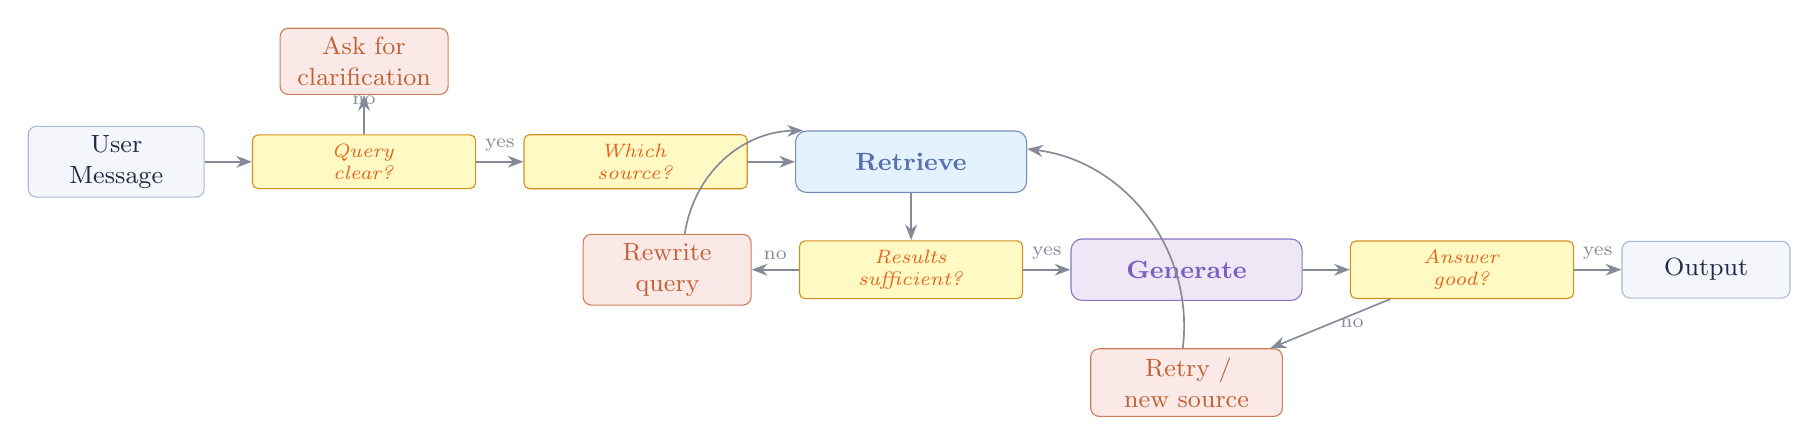
\begin{tikzpicture}[node distance=0.48cm and 0.5cm]
  \node[sbox,text width=2.0cm] (q) {User\\Message};
  \node[dbox,right=0.6cm of q] (dclear) {Query\\clear?};
  \node[fbox,above=0.5cm of dclear,text width=1.9cm] (clarify)
    {Ask for\\clarification};
  \node[dbox,right=0.6cm of dclear] (dsrc) {Which\\source?};
  \node[pbox,right=0.6cm of dsrc] (ret) {Retrieve};
  \node[dbox,below=0.6cm of ret] (dgood) {Results\\sufficient?};
  \node[fbox,left=0.6cm of dgood,text width=1.9cm] (refine) {Rewrite\\query};
  \node[gbox,right=0.6cm of dgood] (llm) {Generate};
  \node[dbox,right=0.6cm of llm] (dok) {Answer\\good?};
  \node[sbox,text width=1.9cm,right=0.6cm of dok] (out) {Output};
  \node[fbox,below=0.6cm of llm,text width=2.2cm] (retry) {Retry /\\new source};

  \draw[arr] (q) -- (dclear);
  \draw[arr] (dclear) -- node[lbl,above] {no} (clarify);
  \draw[arr] (dclear) -- node[lbl,above] {yes} (dsrc);
  \draw[arr] (dsrc) -- (ret);
  \draw[arr] (ret) -- (dgood);
  \draw[arr] (dgood) -- node[lbl,above] {yes} (llm);
  \draw[arr] (dgood) -- node[lbl,above] {no} (refine);
  \draw[arr] (refine) to[bend left=40] (ret);
  \draw[arr] (llm) -- (dok);
  \draw[arr] (dok) -- node[lbl,above] {yes} (out);
  \draw[arr] (dok) -- node[lbl,right] {no} (retry);
  \draw[arr] (retry) to[bend right=45] (ret);
\end{tikzpicture}
\caption{Agentic RAG control loop. The agent (yellow boxes) decides which source to query,
  evaluates whether results are adequate, and retries with a refined query if not.}
\end{figure}

\subsection{Decision Framework: Which Approach to Use?}

\begin{center}
\begin{tabularx}{\linewidth}{lXX}
\toprule
\textbf{Criterion} & \textbf{Standard RAG} & \textbf{Agentic RAG}\\
\midrule
Response latency & 1--3 s & 5--15+ s (multiple LLM calls)\\
Cost per query & $\approx\$0.0002$ & $\approx\$0.001$--$\$0.002$ ($3$--$10\times$)\\
Simple, single-source Q & Excellent & No improvement\\
Complex, multi-source Q & Moderate & Significantly better\\
Debugging & Deterministic, testable & Non-deterministic, hard to reproduce\\
Optimal corpus size & Up to $\sim$10K docs & 10K+ docs, multi-domain\\
\bottomrule
\end{tabularx}
\end{center}

\begin{whybox}
ScholarPath uses \textbf{Standard RAG} for the chatbot.
The corpus has 692 documents and queries are domain-specific (scholarships, consultants,
application tips). A single retrieval pass consistently finds the right document in
$<$10\,ms. Adding an agentic loop would multiply latency by $5\times$ and cost by
$10\times$ with no measurable accuracy gain on this query set.
The threshold for migrating to Agentic RAG is approximately 10,000+ documents
with heterogeneous sub-domains.
\end{whybox}

% ═════════════════════════════════════════════════════════════════════════════
\section{ScholarPath AI Architecture --- The Full Picture}
% ═════════════════════════════════════════════════════════════════════════════

\begin{keybox}{Critical distinction}
ScholarPath has \textbf{three AI features}, but only one uses real RAG + GPT.
The other two use a deterministic, zero-network scoring algorithm.
\end{keybox}

\begin{figure}[H]
\centering
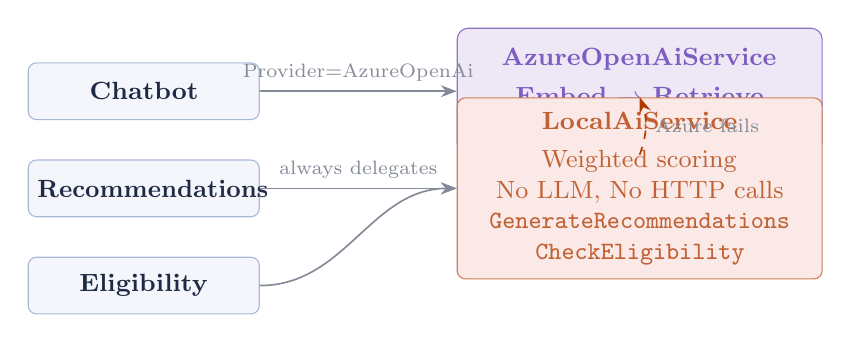
\begin{tikzpicture}[node distance=0.42cm and 0.8cm]
  % Feature boxes (left)
  \node[sbox] (chat) {\textbf{Chatbot}};
  \node[sbox,below=0.5cm of chat] (rec) {\textbf{Recommendations}};
  \node[sbox,below=0.5cm of rec] (eli) {\textbf{Eligibility}};

  % Azure service (top right)
  \node[gbox,right=2.5cm of chat,text width=4.4cm,minimum height=1.6cm] (azure)
    {\textbf{AzureOpenAiService}\\[3pt]
     \small Embed $\rightarrow$ Retrieve\\GPT-4o-mini $\rightarrow$ Answer};

  % Local service (bottom right)
  \node[fbox,right=2.5cm of rec,text width=4.4cm,minimum height=2.3cm] (local)
    {\textbf{LocalAiService}\\[3pt]
     \small Weighted scoring\\No LLM, No HTTP calls\\
     \texttt{GenerateRecommendations}\\
     \texttt{CheckEligibility}};

  \draw[arr] (chat.east) -- node[lbl,above] {Provider=AzureOpenAi} (azure.west);
  \draw[arr] (rec.east) -- node[lbl,above] {always delegates} (local.west);
  \draw[arr] (eli.east) to[out=0,in=180] (local.west);

  % Fallback dashed arrow
  \draw[arrd,color=spSec] (azure.south) to[bend right=20]
    node[lbl,right] {\scriptsize Azure fails} (local.north);
\end{tikzpicture}
\caption{ScholarPath AI routing. The chatbot goes through AzureOpenAiService (real RAG + GPT).
  Recommendations and eligibility always use LocalAiService regardless of the
  \texttt{Ai:Provider} setting.}
\end{figure}

\begin{center}
\begin{tabular}{llll}
\toprule
\textbf{Feature} & \textbf{Uses GPT?} & \textbf{Uses RAG?} & \textbf{Approach}\\
\midrule
Chatbot & \checkmark{} Azure GPT-4o-mini & \checkmark{} Cosine search & Standard RAG\\
Recommendations & $\times$ & $\times$ & Weighted scoring (local)\\
Eligibility & $\times$ & $\times$ & Profile matching (local)\\
\bottomrule
\end{tabular}
\end{center}

\begin{lstlisting}[language={[Sharp]C},caption={AzureOpenAiService.cs --- delegation}]
// Recommendations and eligibility use deterministic scoring, no GPT needed.
public Task<AiRecommendationResult> GenerateRecommendationsAsync(...)
    => local.GenerateRecommendationsAsync(...);  // always LocalAiService

public Task<AiEligibilityResult> CheckEligibilityAsync(...)
    => local.CheckEligibilityAsync(...);         // always LocalAiService

// Only AskAsync uses real Azure RAG + GPT.
public async Task<AiChatResponse> AskAsync(...) { /* RAG pipeline */ }
\end{lstlisting}

% ═════════════════════════════════════════════════════════════════════════════
\section{Knowledge Base --- Building and Maintaining It}
% ═════════════════════════════════════════════════════════════════════════════

\subsection{Five Data Sources}

The \texttt{KnowledgeBaseIndexer.RebuildAsync()} aggregates data from
\textbf{five distinct sources}, each projecting records into a
\texttt{KnowledgeDocument} row in SQL Server:

\begin{figure}[H]
\centering
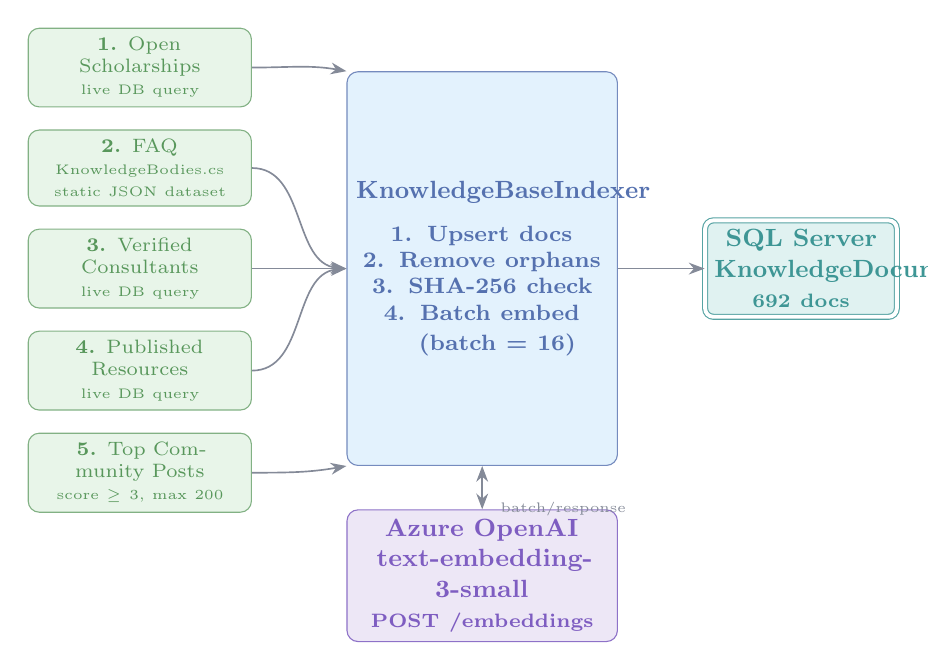
\begin{tikzpicture}[node distance=0.28cm and 1.0cm]
  % Source boxes (left column)
  \node[srcbox] (s1)
    {\textbf{1.} Open Scholarships\\{\tiny live DB query}};
  \node[srcbox,below=0.28cm of s1] (s2)
    {\textbf{2.} FAQ\\{\tiny KnowledgeBodies.cs}\\{\tiny static JSON dataset}};
  \node[srcbox,below=0.28cm of s2] (s3)
    {\textbf{3.} Verified Consultants\\{\tiny live DB query}};
  \node[srcbox,below=0.28cm of s3] (s4)
    {\textbf{4.} Published Resources\\{\tiny live DB query}};
  \node[srcbox,below=0.28cm of s4] (s5)
    {\textbf{5.} Top Community Posts\\{\tiny score $\geq3$, max 200}};

  % Indexer (centre)
  \node[pbox,right=1.2cm of s3,text width=3.2cm,minimum height=5.0cm] (idx)
    {\textbf{KnowledgeBaseIndexer}\\[6pt]
     \footnotesize
     \textbf{1.} Upsert docs\\
     \textbf{2.} Remove orphans\\
     \textbf{3.} SHA-256 check\\
     \textbf{4.} Batch embed\\
     \quad (batch = 16)};

  % Azure Embeddings (below indexer)
  \node[gbox,below=0.55cm of idx,text width=3.2cm] (emb)
    {Azure OpenAI\\text-embedding-3-small\\{\scriptsize POST /embeddings}};

  % SQL DB (right) - double border = database
  \node[dbbox,right=1.1cm of idx,text width=2.2cm] (db)
    {SQL Server\\KnowledgeDocuments\\{\scriptsize 692 docs}};

  % Source arrows
  \draw[arr] (s1.east) to[out=0,in=170] (idx.north west);
  \draw[arr] (s2.east) to[out=0,in=175] (idx.west);
  \draw[arr] (s3.east) -- (idx.west);
  \draw[arr] (s4.east) to[out=0,in=185] (idx.west);
  \draw[arr] (s5.east) to[out=0,in=190] (idx.south west);

  % Indexer to DB
  \draw[arr] (idx.east) -- (db.west);

  % Indexer to Azure (bidirectional)
  \draw[arr,<->] (idx.south) -- (emb.north)
    node[lbl,right=3pt] {\tiny batch/response};
\end{tikzpicture}
\caption{Knowledge base indexer aggregates 5 live data sources. Only documents whose
  content hash has changed (SHA-256 on \texttt{ContentEn + ContentAr}) are re-embedded,
  making incremental rebuilds cheap. Double border = database.}
\end{figure}

\subsection{Rebuild Algorithm}

\begin{enumerate}
  \item \textbf{Upsert} --- For each desired document, compute \texttt{SHA-256(ContentEn+ContentAr)}.
    If the hash changed, clear the embedding. If new, insert.
  \item \textbf{Orphan removal} --- Documents in the DB whose source entity no longer
    exists are deleted.
  \item \textbf{Selective re-embedding} --- Only documents with an empty embedding, a
    model mismatch, or \texttt{force=true} are sent to Azure. On a warm base this is
    zero work.
  \item \textbf{Batch embedding} --- Sent in batches of 16 to
    \texttt{/openai/deployments/text-embedding-3-small/embeddings}.
    The returned \texttt{float[1536]} is packed into \texttt{byte[6144]}
    via \texttt{Buffer.BlockCopy} and stored in a \texttt{VARBINARY} column.
\end{enumerate}

\subsection{Vector Storage --- SQL Server, Not a Vector Database}

\begin{figure}[H]
\centering
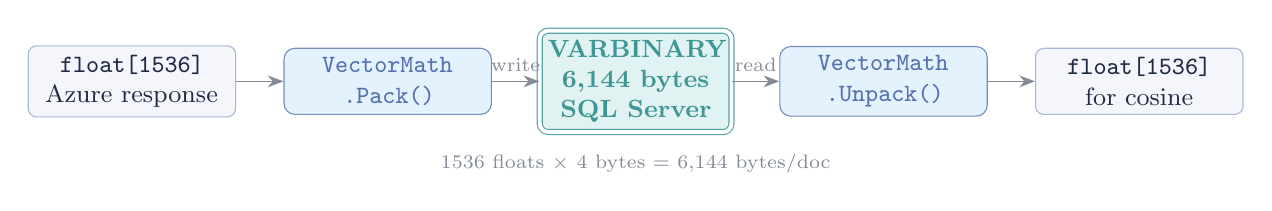
\begin{tikzpicture}[node distance=0.45cm and 0.6cm]
  \node[sbox,text width=2.4cm] (f1) {\texttt{float[1536]}\\Azure response};
  \node[pbox,right=0.6cm of f1,text width=2.4cm] (pack)
    {\texttt{VectorMath}\\\texttt{.Pack()}};
  \node[dbbox,right=0.6cm of pack,text width=2.2cm] (sql)
    {VARBINARY\\6,144 bytes\\SQL Server};
  \node[pbox,right=0.6cm of sql,text width=2.4cm] (unpack)
    {\texttt{VectorMath}\\\texttt{.Unpack()}};
  \node[sbox,text width=2.4cm,right=0.6cm of unpack] (f2)
    {\texttt{float[1536]}\\for cosine};

  \draw[arr] (f1) -- (pack);
  \draw[arr] (pack) -- node[lbl,above] {write} (sql);
  \draw[arr] (sql) -- node[lbl,above] {read} (unpack);
  \draw[arr] (unpack) -- (f2);

  \node[lbl,below=0.15cm of sql] {1536 floats $\times$ 4 bytes $=$ 6,144 bytes/doc};
\end{tikzpicture}
\caption{Zero-copy vector serialisation via \texttt{Buffer.BlockCopy}. SQL Server is
  sufficient at 692 documents --- full in-memory cosine scan completes in $<10$\,ms.}
\end{figure}

\begin{whybox}
A dedicated vector database (Pinecone, Qdrant, pgvector) would add an external
deployment, an additional network hop, and operational cost.
At 692 documents the full in-memory scan is faster than any remote call.
The migration threshold to a vector DB is approximately 10,000--50,000 documents,
where approximate nearest-neighbour (ANN) indexing becomes necessary.
\end{whybox}

% ═════════════════════════════════════════════════════════════════════════════
\section{Chatbot --- Full RAG Pipeline (9 Steps)}
% ═════════════════════════════════════════════════════════════════════════════

\begin{figure}[H]
\centering
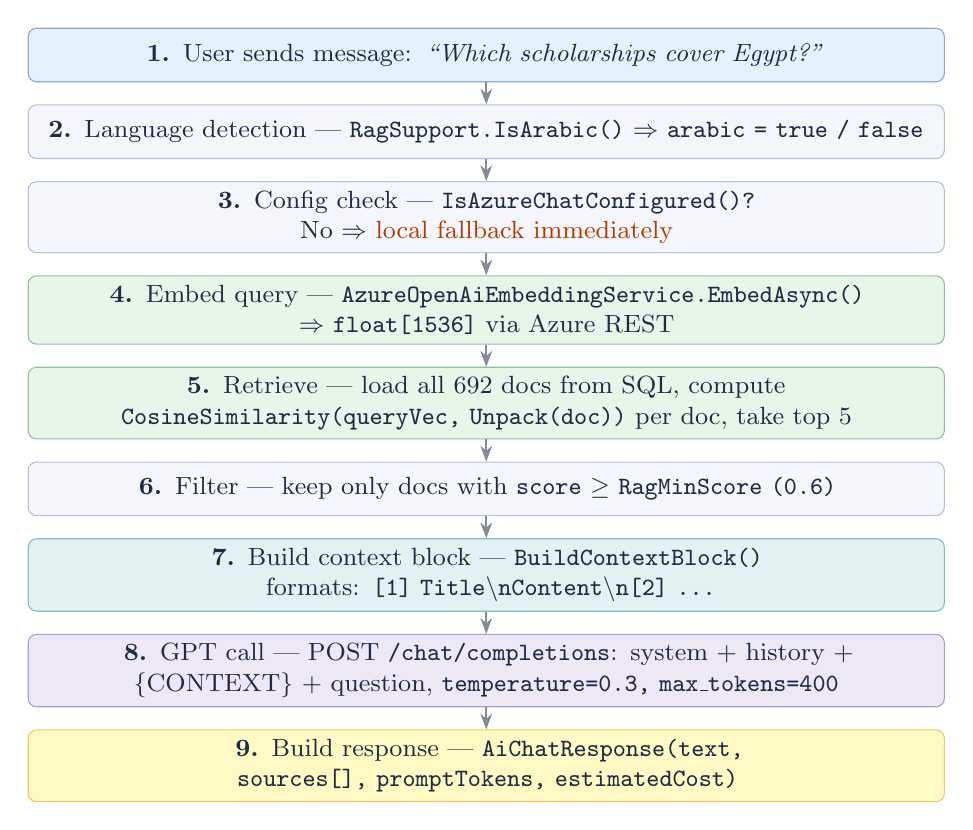
\begin{tikzpicture}[node distance=0.3cm]

  \node[wbox,fill=spLightBlue,draw=spPrimary!50] (s1)
    {\textbf{1.} User sends message: \textit{``Which scholarships cover Egypt?''}};

  \node[wbox,below=0.28cm of s1] (s2)
    {\textbf{2.} Language detection ---
     \texttt{RagSupport.IsArabic()} $\Rightarrow$
     \texttt{arabic = true / false}};

  \node[wbox,below=0.28cm of s2] (s3)
    {\textbf{3.} Config check ---
     \texttt{IsAzureChatConfigured()?}
     \quad No $\Rightarrow$ \textcolor{spSec}{local fallback immediately}};

  \node[wbox,below=0.28cm of s3,fill=spLightGreen,draw=spWhy!50] (s4)
    {\textbf{4.} Embed query ---
     \texttt{AzureOpenAiEmbeddingService.EmbedAsync()} $\Rightarrow$
     \texttt{float[1536]} via Azure REST};

  \node[wbox,below=0.28cm of s4,fill=spLightGreen,draw=spWhy!50] (s5)
    {\textbf{5.} Retrieve --- load all 692 docs from SQL, compute
     \texttt{CosineSimilarity(queryVec, Unpack(doc))} per doc, take top 5};

  \node[wbox,below=0.28cm of s5] (s6)
    {\textbf{6.} Filter ---
     keep only docs with \texttt{score $\geq$ RagMinScore (0.6)}};

  \node[wbox,below=0.28cm of s6,fill=spLightTeal,draw=spAccent!50] (s7)
    {\textbf{7.} Build context block ---
     \texttt{BuildContextBlock()} formats: \texttt{[1] Title{\textbackslash}nContent{\textbackslash}n[2] ...}};

  \node[wbox,below=0.28cm of s7,fill=spLightPurple,draw=spQA!50] (s8)
    {\textbf{8.} GPT call ---
     POST \texttt{/chat/completions}: system + history + \{CONTEXT\} + question,
     \texttt{temperature=0.3, max\_tokens=400}};

  \node[wbox,below=0.28cm of s8,fill=spLightYellow,draw=spYellow!70] (s9)
    {\textbf{9.} Build response ---
     \texttt{AiChatResponse(text, sources[], promptTokens, estimatedCost)}};

  \foreach \from/\to in {s1/s2,s2/s3,s3/s4,s4/s5,s5/s6,s6/s7,s7/s8,s8/s9}
    \draw[arr] (\from) -- (\to);

\end{tikzpicture}
\caption{Complete chatbot pipeline. \colorbox{spLightGreen!60}{Green} steps invoke Azure
  Embeddings API. \colorbox{spLightPurple!60}{Purple} step invokes GPT-4o-mini.
  Total end-to-end latency: $\approx$1--3\,s.}
\end{figure}

\subsection{System Prompt Design}

The system prompt (English and Arabic variants) explicitly instructs the LLM to:

\begin{itemize}
  \item Cite scholarships, consultants, and resources by name when present in the CONTEXT block
  \item Draft SoPs, recommendation letters, CVs, and motivation letters on request
  \item Coach on IELTS/TOEFL/GRE and interview preparation
  \item Explain eligibility requirements and funding mechanics
  \item \textbf{Never} invent scholarship names, deadlines, or amounts not in CONTEXT
  \item \textbf{Never} refuse a reasonable user request
\end{itemize}

\subsection{Session History}

Every API call prepends prior conversation turns between the system prompt and the
current question, giving the model session memory without any server-side store:

\begin{lstlisting}[language={[Sharp]C},caption={ChatCompletionAsync --- session history injection}]
var messages = new List<object>
{
    new { role = "system", content = system },
};
foreach (var turn in history)           // prior turns from this session
    messages.Add(new { role = turn.Role, content = turn.Content });
messages.Add(new { role = "user", content = user });  // current question
\end{lstlisting}

% ═════════════════════════════════════════════════════════════════════════════
\section{Recommendations --- Rule-Based Scoring (No LLM)}
% ═════════════════════════════════════════════════════════════════════════════

\begin{warningbox}
There is \textbf{no GPT call, no RAG, no HTTP request} in the recommendation
pipeline. It is a fully deterministic weighted-scoring algorithm that runs
entirely in-process on the application server.
\end{warningbox}

\subsection{Scoring Formula}

\[
\text{Score}
= \underbrace{S_\text{level}}_{\leq 30}
+ \underbrace{S_\text{field}}_{\leq 40}
+ \underbrace{S_\text{country}}_{\leq 25}
+ \underbrace{B_\text{funding}}_{\leq 5}
\;\in\;[0,\,100]
\]

\begin{figure}[H]
\centering
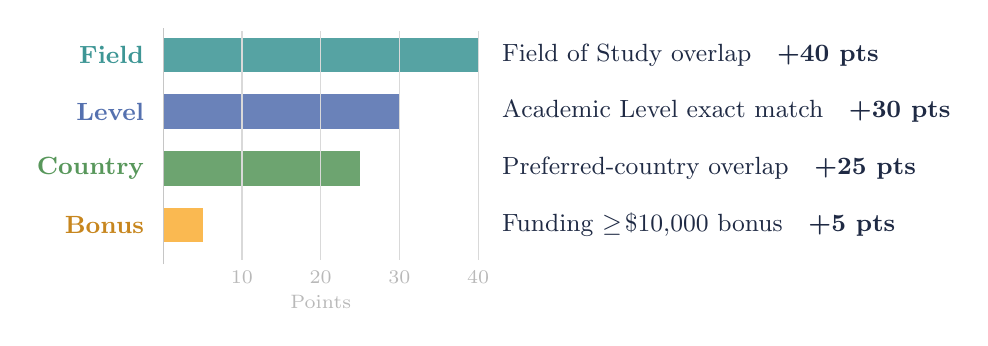
\begin{tikzpicture}
  \def\bh{0.44}
  \def\bg{0.72}

  % Field (40)
  \fill[spAccent!70] (0,0) rectangle (4.0,\bh);
  \node[right,font=\small,text=spInk] at (4.18,\bh/2)
    {Field of Study overlap\quad \textbf{+40 pts}};
  \node[left,font=\small\bfseries,text=spAccent!80] at (-0.12,\bh/2) {Field};

  % Level (30)
  \fill[spPrimary!70] (0,-\bg) rectangle (3.0,-\bg+\bh);
  \node[right,font=\small,text=spInk] at (4.18,-\bg+\bh/2)
    {Academic Level exact match\quad \textbf{+30 pts}};
  \node[left,font=\small\bfseries,text=spPrimary!80] at (-0.12,-\bg+\bh/2) {Level};

  % Country (25)
  \fill[spWhy!70] (0,-2*\bg) rectangle (2.5,-2*\bg+\bh);
  \node[right,font=\small,text=spInk] at (4.18,-2*\bg+\bh/2)
    {Preferred-country overlap\quad \textbf{+25 pts}};
  \node[left,font=\small\bfseries,text=spWhy!80] at (-0.12,-2*\bg+\bh/2) {Country};

  % Bonus (5)
  \fill[spYellow!80] (0,-3*\bg) rectangle (0.5,-3*\bg+\bh);
  \node[right,font=\small,text=spInk] at (4.18,-3*\bg+\bh/2)
    {Funding $\geq\!\$10{,}000$ bonus\quad \textbf{+5 pts}};
  \node[left,font=\small\bfseries,text=spYellow!80!black] at (-0.12,-3*\bg+\bh/2) {Bonus};

  % Axis
  \draw[gray!45,thin] (0,-3*\bg-0.28) -- (0,\bh+0.12);
  \foreach \x/\lbl in {1/10,2/20,3/30,4/40} {
    \draw[gray!30,thin] (\x,-3*\bg-0.22) -- (\x,\bh+0.08);
    \node[font=\scriptsize,gray!55,below] at (\x,-3*\bg-0.24) {\lbl};
  }
  \node[font=\scriptsize,gray!55,below] at (2,-3*\bg-0.55) {Points};
\end{tikzpicture}
\caption{Recommendation score component weights. Field of study is the largest factor
  (40 pts) so subject alignment dominates over geography.}
\end{figure}

\begin{center}
\begin{tabular}{clp{8cm}}
\toprule
\textbf{Score} & \textbf{Label} & \textbf{Explanation shown to student}\\
\midrule
80--100 & Strong match & ``Strong match --- aligns with your preferred fields and level.''\\
50--79  & Partial match & ``Partial match --- overlaps with some of your preferences.''\\
20--49  & Loose match  & ``Loose match --- touches areas you've listed; worth a look.''\\
0--19   & Weak match   & ``Weak match --- doesn't align well with your current profile.''\\
\bottomrule
\end{tabular}
\end{center}

\subsection{Cache Architecture and Re-Hydration}

Scores are computed once and cached as JSON in \texttt{AiInteraction.ResponseText}.
The cached shape (\texttt{RecommendationItemDto}) stores only AI-generated fields.
Live deadline and funding data are \textbf{always fetched fresh from the DB}
so a date change on a scholarship is reflected immediately:

\begin{figure}[H]
\centering
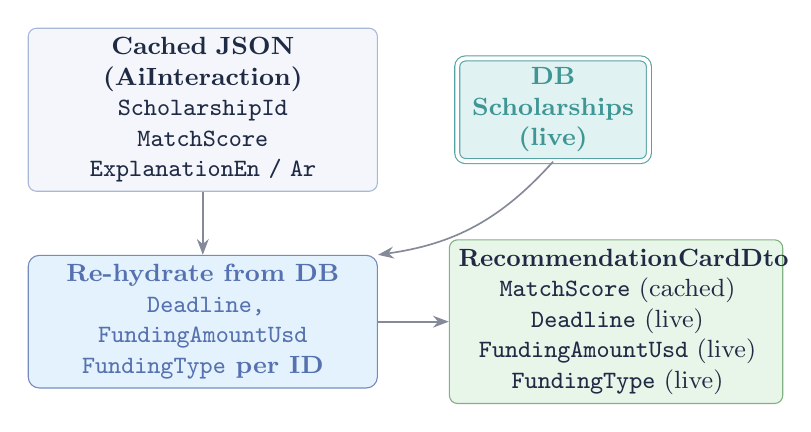
\begin{tikzpicture}[node distance=0.5cm and 0.8cm]
  \node[sbox,text width=4.2cm,align=center] (cache)
    {\textbf{Cached JSON (AiInteraction)}\\
     \texttt{ScholarshipId}\\
     \texttt{MatchScore}\\
     \texttt{ExplanationEn / Ar}};

  \node[dbbox,right=1.0cm of cache,text width=2.2cm] (db)
    {DB\\Scholarships\\(live)};

  \node[pbox,below=0.8cm of cache,text width=4.2cm,align=center] (enrich)
    {Re-hydrate from DB\\
     \texttt{Deadline, FundingAmountUsd}\\
     \texttt{FundingType} per ID};

  \node[sbox,right=0.9cm of enrich,text width=4.0cm,align=center,
    fill=spLightGreen,draw=spWhy!60] (card)
    {\textbf{RecommendationCardDto}\\
     \texttt{MatchScore} (cached)\\
     \texttt{Deadline} (live)\\
     \texttt{FundingAmountUsd} (live)\\
     \texttt{FundingType} (live)};

  \draw[arr] (cache.south) -- (enrich.north);
  \draw[arr] (db.south) to[bend left=20] (enrich.north east);
  \draw[arr] (enrich.east) -- (card.west);
\end{tikzpicture}
\caption{Cache re-hydration. The stored JSON contains only AI-computed fields.
  Deadline and funding are always fetched live so stale dates never appear in the UI.}
\end{figure}

% ═════════════════════════════════════════════════════════════════════════════
\section{Eligibility Check --- Profile Matching}
% ═════════════════════════════════════════════════════════════════════════════

\subsection{Three Criteria}

\begin{center}
\begin{tabular}{llll}
\toprule
\textbf{Criterion} & \textbf{Student source} & \textbf{Scholarship source} & \textbf{Match logic}\\
\midrule
Academic level & \texttt{profile.AcademicLevel} & \texttt{TargetLevel} & Exact equality\\
Country & \texttt{PreferredCountries} + nationality & \texttt{TargetCountriesJson} & \texttt{CountryNormalizer}\\
Field of study & \texttt{profile.FieldOfStudy} & \texttt{FieldsOfStudyJson} & Case-insensitive contains\\
\bottomrule
\end{tabular}
\end{center}

Per-criterion match values: \texttt{"yes"} / \texttt{"partial"} / \texttt{"no"} /
\texttt{"unknown"} (when the student's profile field is empty).

\subsection{Verdict Derivation}

\begin{figure}[H]
\centering
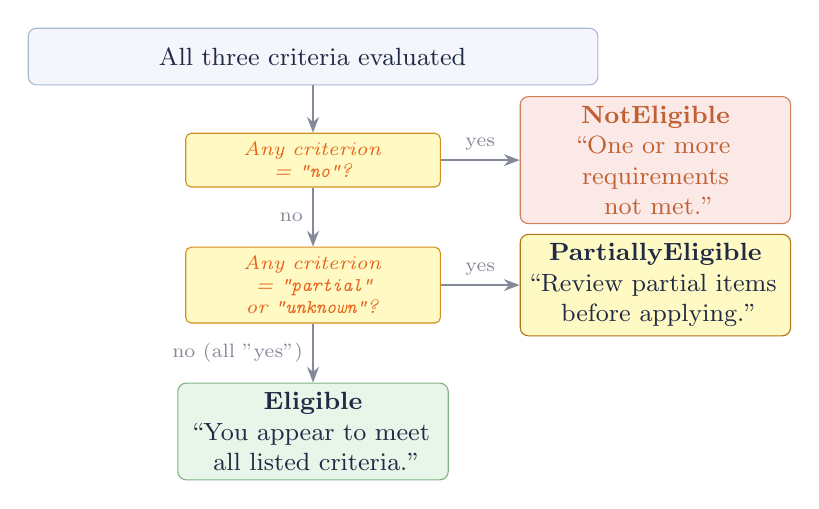
\begin{tikzpicture}[node distance=0.52cm and 0.75cm]
  \node[sbox,text width=7.0cm] (start)
    {All three criteria evaluated};

  \node[dbox,below=0.6cm of start,text width=3.0cm] (hasno)
    {Any criterion\\= \texttt{"no"}?};

  \node[fbox,right=1.0cm of hasno,text width=3.2cm] (nope)
    {\textbf{NotEligible}\\
     \small ``One or more requirements\\not met.''};

  \node[dbox,below=0.75cm of hasno,text width=3.0cm] (hasprt)
    {Any criterion\\= \texttt{"partial"}\\or \texttt{"unknown"}?};

  \node[sbox,right=1.0cm of hasprt,text width=3.2cm,
    fill=spLightYellow,draw=spYellow!70!black] (part)
    {\textbf{PartiallyEligible}\\
     \small ``Review partial items\\before applying.''};

  \node[sbox,below=0.75cm of hasprt,text width=3.2cm,
    fill=spLightGreen,draw=spWhy!60] (elig)
    {\textbf{Eligible}\\
     \small ``You appear to meet\\all listed criteria.''};

  \draw[arr] (start) -- (hasno);
  \draw[arr] (hasno) -- node[lbl,above] {yes} (nope);
  \draw[arr] (hasno) -- node[lbl,left] {no} (hasprt);
  \draw[arr] (hasprt) -- node[lbl,above] {yes} (part);
  \draw[arr] (hasprt) -- node[lbl,left] {no (all "yes")} (elig);
\end{tikzpicture}
\caption{Verdict derivation in \texttt{LocalAiService.DeriveVerdict()}.
  A single ``no'' is sufficient for \texttt{NotEligible};
  any uncertainty yields \texttt{PartiallyEligible}.}
\end{figure}

\begin{notebox}
\textbf{Country normalisation} is non-trivial.
A scholarship listing ``France'' must match a student who typed ``FR'', ``france'',
or ``France''.
\texttt{CountryNormalizer.Matches()} collapses all representations to a canonical key
before comparison.
Without this, an Egyptian student preferring Germany would read ``no''
on a scholarship listing the country as ``DE''.
\end{notebox}

% ═════════════════════════════════════════════════════════════════════════════
\section{Fallback Chain --- Graceful Degradation}
% ═════════════════════════════════════════════════════════════════════════════

Every AI call is wrapped in a multi-level fallback that ensures the user
always receives a response, even if Azure is completely unreachable.

\begin{figure}[H]
\centering
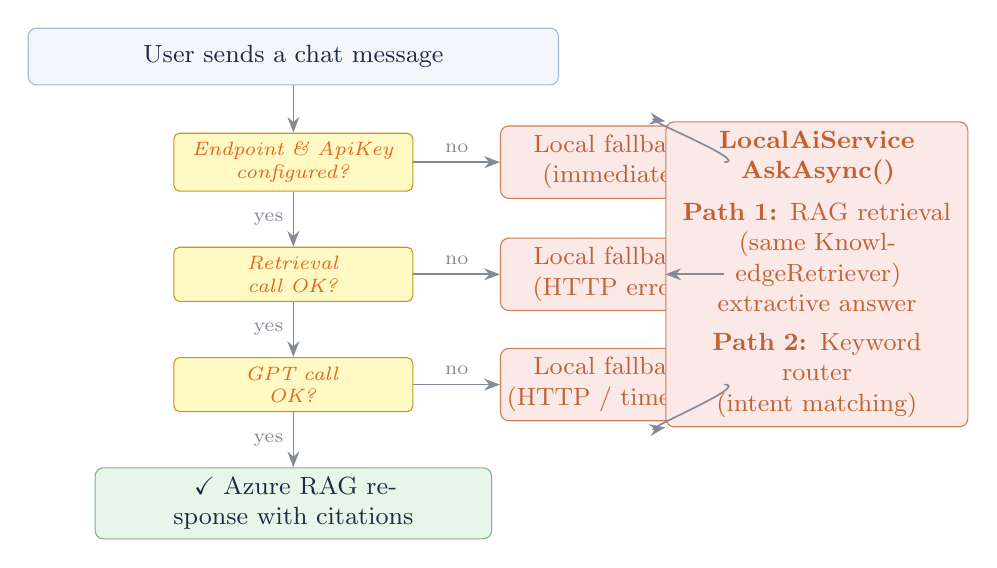
\begin{tikzpicture}[node distance=0.52cm and 0.75cm]
  \node[sbox,text width=6.5cm] (req) {User sends a chat message};

  \node[dbox,below=0.6cm of req,text width=2.8cm] (c1)
    {Endpoint \& ApiKey\\configured?};
  \node[fbox,right=1.1cm of c1,text width=2.6cm] (f1)
    {Local fallback\\(immediate)};

  \node[dbox,below=0.7cm of c1,text width=2.8cm] (c2)
    {Retrieval\\call OK?};
  \node[fbox,right=1.1cm of c2,text width=2.6cm] (f2)
    {Local fallback\\(HTTP error)};

  \node[dbox,below=0.7cm of c2,text width=2.8cm] (c3)
    {GPT call\\OK?};
  \node[fbox,right=1.1cm of c3,text width=2.6cm] (f3)
    {Local fallback\\(HTTP / timeout)};

  \node[sbox,below=0.7cm of c3,text width=4.8cm,fill=spLightGreen,
    draw=spWhy!60] (ok)
    {\checkmark{} Azure RAG response with citations};

  % Main local service block
  \node[fbox,right=3.2cm of c2,text width=3.6cm,minimum height=3.8cm] (local)
    {\textbf{LocalAiService}\\
     \textbf{AskAsync()}\\[4pt]
     \small \textbf{Path 1:} RAG retrieval\\(same KnowledgeRetriever)\\extractive answer\\[3pt]
     \textbf{Path 2:} Keyword\\router\\(intent matching)};

  \draw[arr] (req) -- (c1);
  \draw[arr] (c1) -- node[lbl,left] {yes} (c2);
  \draw[arr] (c1) -- node[lbl,above] {no} (f1);
  \draw[arr] (c2) -- node[lbl,left] {yes} (c3);
  \draw[arr] (c2) -- node[lbl,above] {no} (f2);
  \draw[arr] (c3) -- node[lbl,left] {yes} (ok);
  \draw[arr] (c3) -- node[lbl,above] {no} (f3);

  \draw[arr] (f1.east) to[out=0,in=170] (local.north west);
  \draw[arr] (f2.east) -- (local.west);
  \draw[arr] (f3.east) to[out=0,in=190] (local.south west);
\end{tikzpicture}
\caption{Three-level fallback chain for the chatbot.
  Any failure routes to \texttt{LocalAiService.AskAsync()}, which runs the same
  RAG retrieval without GPT, then falls back to a keyword router.}
\end{figure}

% ═════════════════════════════════════════════════════════════════════════════
\section{Cost Model and Fine-Tuning Roadmap}
% ═════════════════════════════════════════════════════════════════════════════

\subsection{Production Cost (GPT-4o-mini)}

\[
\text{Cost}
= N_\text{prompt} \times \frac{\$0.15}{10^6}
+ N_\text{completion} \times \frac{\$0.60}{10^6}
\]

\begin{center}
\begin{tabular}{lrrr}
\toprule
\textbf{Scenario} & \textbf{Prompt tok.} & \textbf{Completion tok.} & \textbf{Cost}\\
\midrule
Simple chat turn & 300 & 150 & $\approx\$0.000135$\\
Rich context (5 docs retrieved) & 600 & 300 & $\approx\$0.000270$\\
1,000 turns/day & --- & --- & $\approx\$0.27$\\
\texttt{DailyCostLimitUsd} cap & \multicolumn{3}{l}{\$5.00 --- hard limit in \texttt{AiOptions}}\\
\bottomrule
\end{tabular}
\end{center}

\subsection{Fine-Tuning Roadmap}

A fine-tuning dataset (\texttt{scholarpath-finetune.jsonl}, 332 training examples)
has been generated in OpenAI chat format. The codebase already contains the
selection logic --- no code change is required to activate it:

\begin{lstlisting}[language={[Sharp]C},caption={Automatic fine-tuned model selection}]
var deployment = string.IsNullOrWhiteSpace(az.FineTunedDeploymentName)
    ? az.DeploymentName           // "gpt-4o-mini"  (current)
    : az.FineTunedDeploymentName; // e.g. "scholarpath-ft-001"
\end{lstlisting}

Setting the App Service environment variable
\texttt{Ai\_\_AzureOpenAi\_\_FineTunedDeploymentName} is sufficient to switch models.

% ═════════════════════════════════════════════════════════════════════════════
\section{Admin Knowledge Base Management}
% ═════════════════════════════════════════════════════════════════════════════

\subsection{Four Actions on the Admin Page}

The page \texttt{AdminKnowledgeBase.tsx} exposes four operations on the knowledge base,
each wired to a dedicated API endpoint:

\begin{center}
\begin{tabular}{p{3.0cm}p{5.8cm}p{4.4cm}}
\toprule
\textbf{Button} & \textbf{API call} & \textbf{Effect}\\
\midrule
Rebuild (incremental) &
  \texttt{POST .../knowledge-base/rebuild?force=false} &
  Re-embeds only changed docs\\
Rebuild (force) &
  \texttt{POST .../knowledge-base/rebuild?force=true} &
  Re-embeds ALL 692 docs\\
Import + Rebuild &
  \texttt{POST .../datasets/import} &
  Fetches external scholarships, then rebuilds\\
Export Fine-Tuning &
  \texttt{GET .../fine-tuning/dataset} &
  Downloads \texttt{scholarpath-finetune.jsonl}\\
\bottomrule
\end{tabular}
\end{center}

The rebuild response is a \texttt{KnowledgeBaseRebuildResultDto}:

\begin{lstlisting}[language={},caption={Admin UI receives this on every rebuild}]
{
  "upserted":    12,   // new or content-changed docs saved to DB
  "reembedded":   3,   // docs whose embedding was refreshed (hash changed)
  "removed":      2    // orphan docs deleted (source entity no longer exists)
}
\end{lstlisting}

\subsection{Incremental vs.\ Force Rebuild}

\begin{figure}[H]
\centering
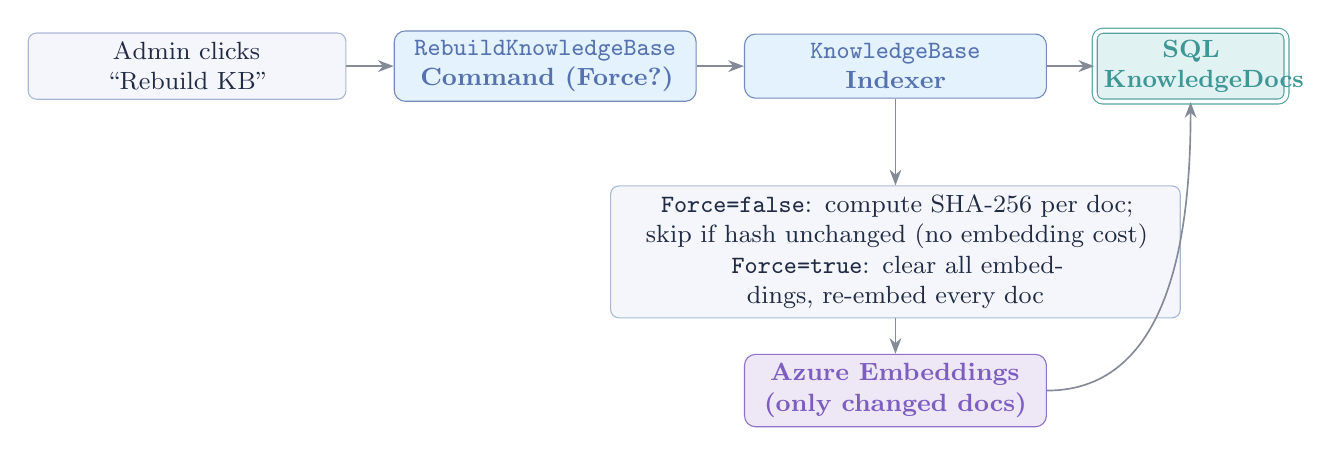
\begin{tikzpicture}[node distance=0.3cm and 0.55cm]
  \node[sbox,text width=3.8cm] (admin) {Admin clicks\\``Rebuild KB''};
  \node[pbox,right=0.6cm of admin,text width=3.6cm] (cmd)
    {\texttt{RebuildKnowledgeBase}\\Command (Force?)};
  \node[pbox,right=0.6cm of cmd,text width=3.6cm] (idx)
    {\texttt{KnowledgeBase}\\Indexer};
  \node[dbbox,right=0.6cm of idx,text width=2.2cm] (db)
    {SQL\\KnowledgeDocs};

  \node[sbox,below=1.1cm of idx,text width=7.0cm] (logic)
    {\texttt{Force=false}: compute SHA-256 per doc;
     skip if hash unchanged (no embedding cost)\\
     \texttt{Force=true}: clear all embeddings, re-embed every doc};

  \node[gbox,below=0.45cm of logic,text width=3.6cm] (az)
    {Azure Embeddings\\(only changed docs)};

  \draw[arr] (admin) -- (cmd);
  \draw[arr] (cmd) -- (idx);
  \draw[arr] (idx) -- (db);
  \draw[arr] (idx.south) -- (logic.north);
  \draw[arr] (logic.south) -- (az.north);
  \draw[arr] (az.east) to[out=0,in=270] (db.south);
\end{tikzpicture}
\caption{Rebuild decision flow. \texttt{Force=false} is the default --- only documents
  whose \texttt{SHA-256(ContentEn + ContentAr)} changed are sent to Azure.
  A warm rebuild typically costs \$0.00 in embedding tokens.}
\end{figure}

\begin{whybox}
The SHA-256 check makes nightly Hangfire-triggered rebuilds essentially free.
Changing one scholarship's description re-embeds exactly one document (1,536 floats =
\$0.000002). A force rebuild re-embeds all 692 documents
(cost: $692 \times 1536 \times \$0.02/10^6 \approx \$0.021$).
\end{whybox}

% ═════════════════════════════════════════════════════════════════════════════
\section{Fine-Tuning Pipeline (In-App)}
% ═════════════════════════════════════════════════════════════════════════════

Fine-tuning in ScholarPath is fully managed from the admin panel --- no
PowerShell scripts, no manual file uploads. The pipeline covers four steps:
export, upload, train, and activate.

% ─────────────────────────────────────────────────────────────────────────────
\subsection{JSONL Dataset Generation}
% ─────────────────────────────────────────────────────────────────────────────

The \textbf{Export Fine-Tuning} button downloads \texttt{scholarpath-finetune.jsonl} ---
a supervised fine-tuning dataset in OpenAI chat-completion format.
It is generated on-demand by \texttt{ExportFineTuningDatasetQueryHandler} with no
external calls: all data comes from the live database and
the static \texttt{KnowledgeBodies.cs} constant.

Each line is one self-contained training example:

\begin{lstlisting}[language={},caption={Single JSONL training example (truncated)}]
{
  "messages": [
    {
      "role": "system",
      "content": "You are ScholarPath AI, a bilingual assistant..."
    },
    {
      "role": "user",
      "content": "Tell me about the Erasmus+ scholarship."
    },
    {
      "role": "assistant",
      "content": "The Erasmus+ scholarship is a European Union programme
                  that supports student mobility..."
    }
  ]
}
\end{lstlisting}

\begin{center}
\begin{tabular}{llr}
\toprule
\textbf{Source} & \textbf{Example type} & \textbf{Count (approx.)}\\
\midrule
\texttt{KnowledgeBodies.cs} & FAQ English Q\&A pairs & $\sim$32\\
\texttt{KnowledgeBodies.cs} & FAQ Arabic Q\&A pairs & $\sim$32\\
Open Scholarships (DB) & Overview in English & $\leq$100\\
Open Scholarships (DB) & Overview in Arabic & $\leq$100\\
Open Scholarships (DB) & Eligibility requirements & $\leq$68\\
\midrule
\textbf{Total} & & $\sim$332\\
\bottomrule
\end{tabular}
\end{center}

% ─────────────────────────────────────────────────────────────────────────────
\subsection{Starting a Fine-Tuning Job from the Admin Panel}
% ─────────────────────────────────────────────────────────────────────────────

The admin clicks \textbf{Start fine-tuning job} on the Knowledge Base page.
Under the hood \texttt{StartFineTuningJobCommand} performs three steps in one
HTTP call:

\begin{enumerate}
  \item Calls \texttt{ExportFineTuningDatasetQuery} internally to obtain the JSONL.
  \item Uploads the file to the Azure OpenAI Files API
        (\texttt{POST /openai/files}) via \texttt{AzureFineTuningService},
        then polls \texttt{GET /openai/files/\{id\}} until \texttt{status = "processed"}.
  \item Creates the fine-tuning job:
        \texttt{POST /openai/fine\_tuning/jobs}
        with \texttt{model = "gpt-4o-mini"} and the uploaded \texttt{training\_file} ID.
\end{enumerate}

The resulting \texttt{jobId} and initial status \texttt{"submitted"} are persisted
in the \texttt{PlatformSettings} table under the keys shown below.
The job runs asynchronously on Azure (typically 30--90 minutes).

\begin{lstlisting}[language={},caption={PlatformSettings keys for fine-tuning state}]
ai.fineTuning.lastJobId            -- Azure job ID (e.g. "ftjob-abc123")
ai.fineTuning.lastJobStatus        -- last-known status string
ai.fineTuning.lastFinishedModel    -- model name once the job succeeds
ai.fineTuning.activeDeploymentName -- currently active fine-tuned deployment
\end{lstlisting}

% ─────────────────────────────────────────────────────────────────────────────
\subsection{Checking Job Status}
% ─────────────────────────────────────────────────────────────────────────────

The admin clicks \textbf{Check status} (or the client polls automatically).
\texttt{GetFineTuningJobStatusQuery} reads the stored \texttt{jobId} from
\texttt{PlatformSettings}, calls
\texttt{GET /openai/fine\_tuning/jobs/\{id\}} on Azure,
writes the fresh status back to \texttt{PlatformSettings}, and returns:

\begin{lstlisting}[language={[Sharp]C},caption={FineTuningStatusDto returned by GET /api/admin/ai/fine-tuning/status}]
public sealed record FineTuningStatusDto(
    string?  JobId,
    string   Status,          // "submitted" | "running" | "succeeded" | "failed"
    string?  FineTunedModel,  // model name once succeeded
    string?  Error,
    string?  ActiveDeploymentName,
    bool     HasActiveDeployment);
\end{lstlisting}

% ─────────────────────────────────────────────────────────────────────────────
\subsection{Activating the Fine-Tuned Model}
% ─────────────────────────────────────────────────────────────────────────────

Once the job status is \texttt{"succeeded"} and the admin has created a deployment
in Azure AI Foundry from the finished model, they enter the deployment name in the
admin panel and click \textbf{Activate}.

\texttt{ActivateFineTunedModelCommand} writes the deployment name to
\texttt{PlatformSettings("ai.fineTuning.activeDeploymentName")}.
No App Service restart is required.

\texttt{AzureOpenAiService} resolves the deployment on every chat call using this
three-tier priority:

\begin{lstlisting}[language={[Sharp]C},caption={Deployment selection in AzureOpenAiService.cs}]
// Priority: DB platform setting -> appsettings override -> base model
var dbDeployment = await PlatformSettingsReader.GetStringAsync(
    db, PlatformSettingsKeys.ActiveFineTunedDeploymentName, null, ct);
var deployment = !string.IsNullOrWhiteSpace(dbDeployment)
    ? dbDeployment
    : !string.IsNullOrWhiteSpace(az.FineTunedDeploymentName)
        ? az.FineTunedDeploymentName
        : az.DeploymentName;
\end{lstlisting}

The admin can also click \textbf{Revert to base model} to clear the
platform-setting and restore \texttt{gpt-4o-mini} immediately.

% ─────────────────────────────────────────────────────────────────────────────
\subsection{Admin API Endpoints}
% ─────────────────────────────────────────────────────────────────────────────

\begin{center}
\begin{tabular}{lll}
\toprule
\textbf{Method} & \textbf{Route} & \textbf{Purpose}\\
\midrule
\texttt{GET}    & \texttt{/api/admin/ai/fine-tuning/dataset}  & Export JSONL (download)\\
\texttt{POST}   & \texttt{/api/admin/ai/fine-tuning/start}    & Upload + start job\\
\texttt{GET}    & \texttt{/api/admin/ai/fine-tuning/status}   & Poll job status\\
\texttt{PUT}    & \texttt{/api/admin/ai/fine-tuning/activate} & Set active deployment\\
\texttt{DELETE} & \texttt{/api/admin/ai/fine-tuning/activate} & Revert to base model\\
\bottomrule
\end{tabular}
\end{center}

% ═════════════════════════════════════════════════════════════════════════════
\section{AiInteraction Entity --- The Caching Layer}
% ═════════════════════════════════════════════════════════════════════════════

\subsection{Entity Structure}

\texttt{AiInteraction} is the \textbf{single table for all AI operations} ---
it serves as both an audit log and a cache.

\begin{lstlisting}[language={[Sharp]C},caption={Domain/Entities/AI.cs (condensed)}]
public class AiInteraction : AuditableEntity
{
    public Guid     UserId          { get; set; }
    public AiFeature Feature        { get; set; }  // Recommendation | Chat | Eligibility
    public AiProvider Provider      { get; set; }  // AzureOpenAi | Local
    public string?  SessionId       { get; set; }  // groups chat turns into a session

    // The payload -- meaning varies by Feature:
    public string   PromptText      { get; set; }  // what was asked
    public string   ResponseText    { get; set; }  // answer text OR cached JSON
    public string?  MetadataJson    { get; set; }  // structured breakdown (eligibility)

    // Billing
    public int      PromptTokens    { get; set; }
    public int      CompletionTokens{ get; set; }
    public decimal  CostUsd         { get; set; }

    public DateTimeOffset StartedAt   { get; set; }
    public DateTimeOffset? CompletedAt{ get; set; }
    public string?  ErrorMessage    { get; set; }
}
\end{lstlisting}

\subsection{ResponseText by Feature}

\begin{center}
\begin{tabular}{lp{5.5cm}p{5.0cm}}
\toprule
\textbf{Feature} & \textbf{ResponseText content} & \textbf{Read by}\\
\midrule
\texttt{Recommendation} &
  \texttt{List<RecommendationItemDto>} as JSON &
  \texttt{GetMyRecommendationsQuery}\\
\texttt{Chat} &
  Plain assistant reply text &
  \texttt{GetAiSessionTurnsQuery}\\
\texttt{Eligibility} &
  Verdict string; detail in \texttt{MetadataJson} &
  Client displays directly\\
\bottomrule
\end{tabular}
\end{center}

\subsection{Full Recommendation Cache Lifecycle}

\begin{figure}[H]
\centering
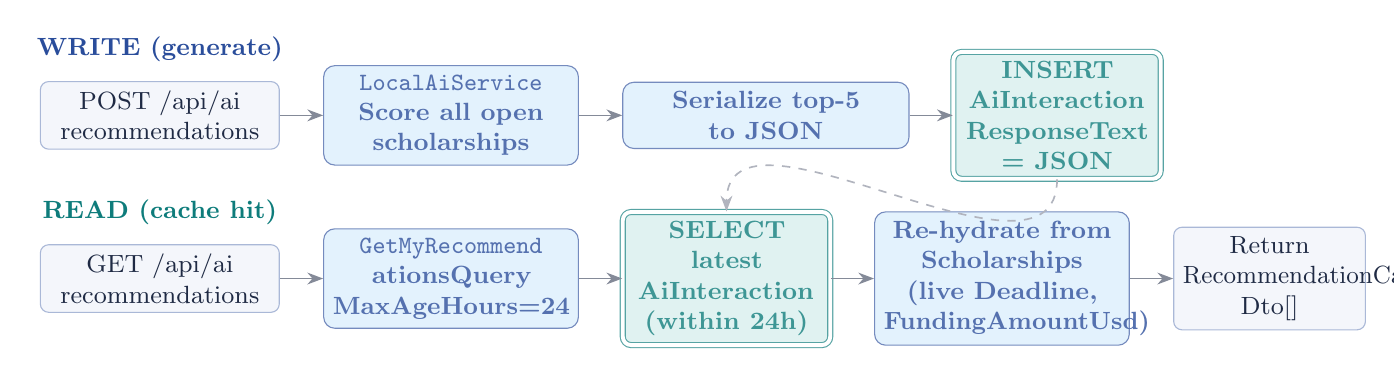
\begin{tikzpicture}[node distance=0.32cm and 0.55cm]
  %% --- WRITE PATH ---
  \node[sbox,text width=2.8cm] (post) {POST /api/ai\\recommendations};
  \node[pbox,right=0.55cm of post,text width=3.0cm] (score)
    {\texttt{LocalAiService}\\Score all open\\scholarships};
  \node[pbox,right=0.55cm of score,text width=3.4cm] (ser)
    {Serialize top-5\\to JSON};
  \node[dbbox,right=0.55cm of ser,text width=2.4cm] (db)
    {INSERT\\AiInteraction\\ResponseText = JSON};

  \node[font=\small\bfseries,color=spPrimary,above=0.12cm of post] {WRITE (generate)};

  \draw[arr] (post) -- (score);
  \draw[arr] (score) -- (ser);
  \draw[arr] (ser) -- (db);

  %% --- READ PATH ---
  \node[sbox,text width=2.8cm,below=1.2cm of post] (get)
    {GET /api/ai\\recommendations};
  \node[pbox,right=0.55cm of get,text width=3.0cm] (qry)
    {\texttt{GetMyRecommend}\\ationsQuery\\MaxAgeHours=24};
  \node[dbbox,right=0.55cm of qry,text width=2.4cm] (read)
    {SELECT latest\\AiInteraction\\(within 24h)};
  \node[pbox,right=0.55cm of read,text width=3.0cm] (hydrate)
    {Re-hydrate from\\Scholarships\\(live Deadline,\\FundingAmountUsd)};
  \node[sbox,right=0.55cm of hydrate,text width=2.2cm] (resp)
    {Return\\RecommendationCard\\Dto[]};

  \node[font=\small\bfseries,color=spAccent,above=0.12cm of get] {READ (cache hit)};

  \draw[arr] (get) -- (qry);
  \draw[arr] (qry) -- (read);
  \draw[arr] (read) -- (hydrate);
  \draw[arr] (hydrate) -- (resp);

  % Connect the two paths through the DB
  \draw[arrd] (db.south) to[out=270,in=90] (read.north);
\end{tikzpicture}
\caption{Recommendation cache lifecycle. The write path (generate) runs once and stores scored
  items as JSON. The read path (cache hit) deserialises the JSON and re-hydrates live
  deadline/funding data so stale values never appear in the UI.
  \texttt{MaxAgeHours=24} --- cached results older than 24 h are treated as missing and
  trigger a fresh generation.}
\end{figure}

\subsection{Related Entities}

\begin{center}
\begin{tabular}{lp{9cm}}
\toprule
\textbf{Entity} & \textbf{Purpose}\\
\midrule
\texttt{RecommendationClickEvent} &
  Logged when user clicks a recommendation card. Tracks
  \texttt{Source} (``card'', ``email'', etc.) for CTR analysis.\\
\texttt{AiRedactionAuditSample} &
  Monthly PII-redaction compliance sample --- stores a
  random chat turn and verifies no personal data leaked into responses.\\
\bottomrule
\end{tabular}
\end{center}

% ═════════════════════════════════════════════════════════════════════════════
\section{Configuration Reference}
% ═════════════════════════════════════════════════════════════════════════════

\begin{center}
\begin{tabular}{lll}
\toprule
\textbf{Setting key} & \textbf{Production value} & \textbf{Effect}\\
\midrule
\texttt{Ai:Provider} & \texttt{AzureOpenAi} & Route chatbot through Azure\\
\texttt{Ai:RagTopK} & \texttt{5} & Maximum documents retrieved per query\\
\texttt{Ai:RagMinScore} & \texttt{0.6} & Minimum cosine similarity to include a doc\\
\texttt{Ai:DailyCostLimitUsd} & \texttt{5.0} & Hard daily spend cap\\
\texttt{AzureOpenAi:DeploymentName} & \texttt{gpt-4o-mini} & Chat generation model\\
\texttt{AzureOpenAi:EmbeddingDeploymentName} & \texttt{text-embedding-3-small} & Embedding model\\
\texttt{AzureOpenAi:EmbeddingDimensions} & \texttt{1536} & Vector size\\
\texttt{AzureOpenAi:FineTunedDeploymentName} & \texttt{(empty)} & Post-launch fine-tuned model\\
\bottomrule
\end{tabular}
\end{center}

% ═════════════════════════════════════════════════════════════════════════════
\section{Summary}
% ═════════════════════════════════════════════════════════════════════════════

\begin{keybox}{One-sentence summary per feature}
\textbf{Chatbot:}
user message $\rightarrow$ Azure Embed $\rightarrow$ cosine search (692 docs, in-memory)
$\rightarrow$ top-5 docs filtered at 0.6 $\rightarrow$ GPT-4o-mini with context
$\rightarrow$ cited answer.

\medskip
\textbf{Recommendations:}
student profile $\rightarrow$ weighted score per open scholarship
(level 30 + field 40 + country 25 + bonus 5) $\rightarrow$ top-5 ranked list;
cached as JSON, deadline/funding re-hydrated from DB on every read.

\medskip
\textbf{Eligibility:}
student profile vs.\ scholarship criteria $\rightarrow$ yes/partial/no per criterion
$\rightarrow$ \texttt{Eligible} / \texttt{PartiallyEligible} / \texttt{NotEligible} verdict.
\end{keybox}

\begin{center}
\begin{tabular}{llll}
\toprule
\textbf{Feature} & \textbf{Uses GPT?} & \textbf{Uses RAG?} & \textbf{Approach}\\
\midrule
Chatbot & \checkmark{} Azure GPT-4o-mini & \checkmark{} Cosine search & Standard RAG\\
Recommendations & $\times$ & $\times$ & Weighted scoring (deterministic)\\
Eligibility & $\times$ & $\times$ & Profile matching (deterministic)\\
\bottomrule
\end{tabular}
\end{center}

\bigskip
\noindent\small
\textbf{Primary reference.}
ByteByteGo, \textit{How Agentic RAG Works},
\url{https://blog.bytebytego.com/p/how-agentic-rag-works}.

\noindent
\textbf{Implementation.}
\texttt{server/src/ScholarPath.Infrastructure/Services/}
(\texttt{AzureOpenAiService.cs}, \texttt{KnowledgeBaseIndexer.cs},
\texttt{KnowledgeRetriever.cs}, \texttt{LocalAiService.cs},
\texttt{VectorMath.cs}, \texttt{RagSupport.cs}).

\end{document}
